\documentclass[11pt,english]{article}
\usepackage[T1]{fontenc}
\usepackage{babel}
\usepackage{graphicx}
\usepackage{epstopdf}
\usepackage[top=1in, bottom=1in, left=0.5in, right=0.5in]{geometry}
\usepackage{amsmath}
\usepackage{natbib}

\author{
  Pratyaksh Sharma\\
  120050019\\
  pratyaksh@cse.iitb.ac.in
  \and
  Sanket Kanjanlkar\\
  120050011\\
  sanket@cse.iitb.ac.in
  \and 
  Shirish Namdeo\\
  110050040\\
  shirishkumar@cse.iitb.ac.in
}
\title{Physics Behind the Simulation: A CS296 Report by Group 09}
\date{25 January, 2014}

\begin{document}
\maketitle

  \section{Introduction}
\indent
\par{This document explains the working of the components added to the Box2D simulation given in cs296\_base\_code. The physics governing the motion of these components is described and relevant images have been added.\\ \indent Various references for further reading are also mentioned.}


\section{Physics behind the simulation.}

\begin{figure}[h!]
  \centering
    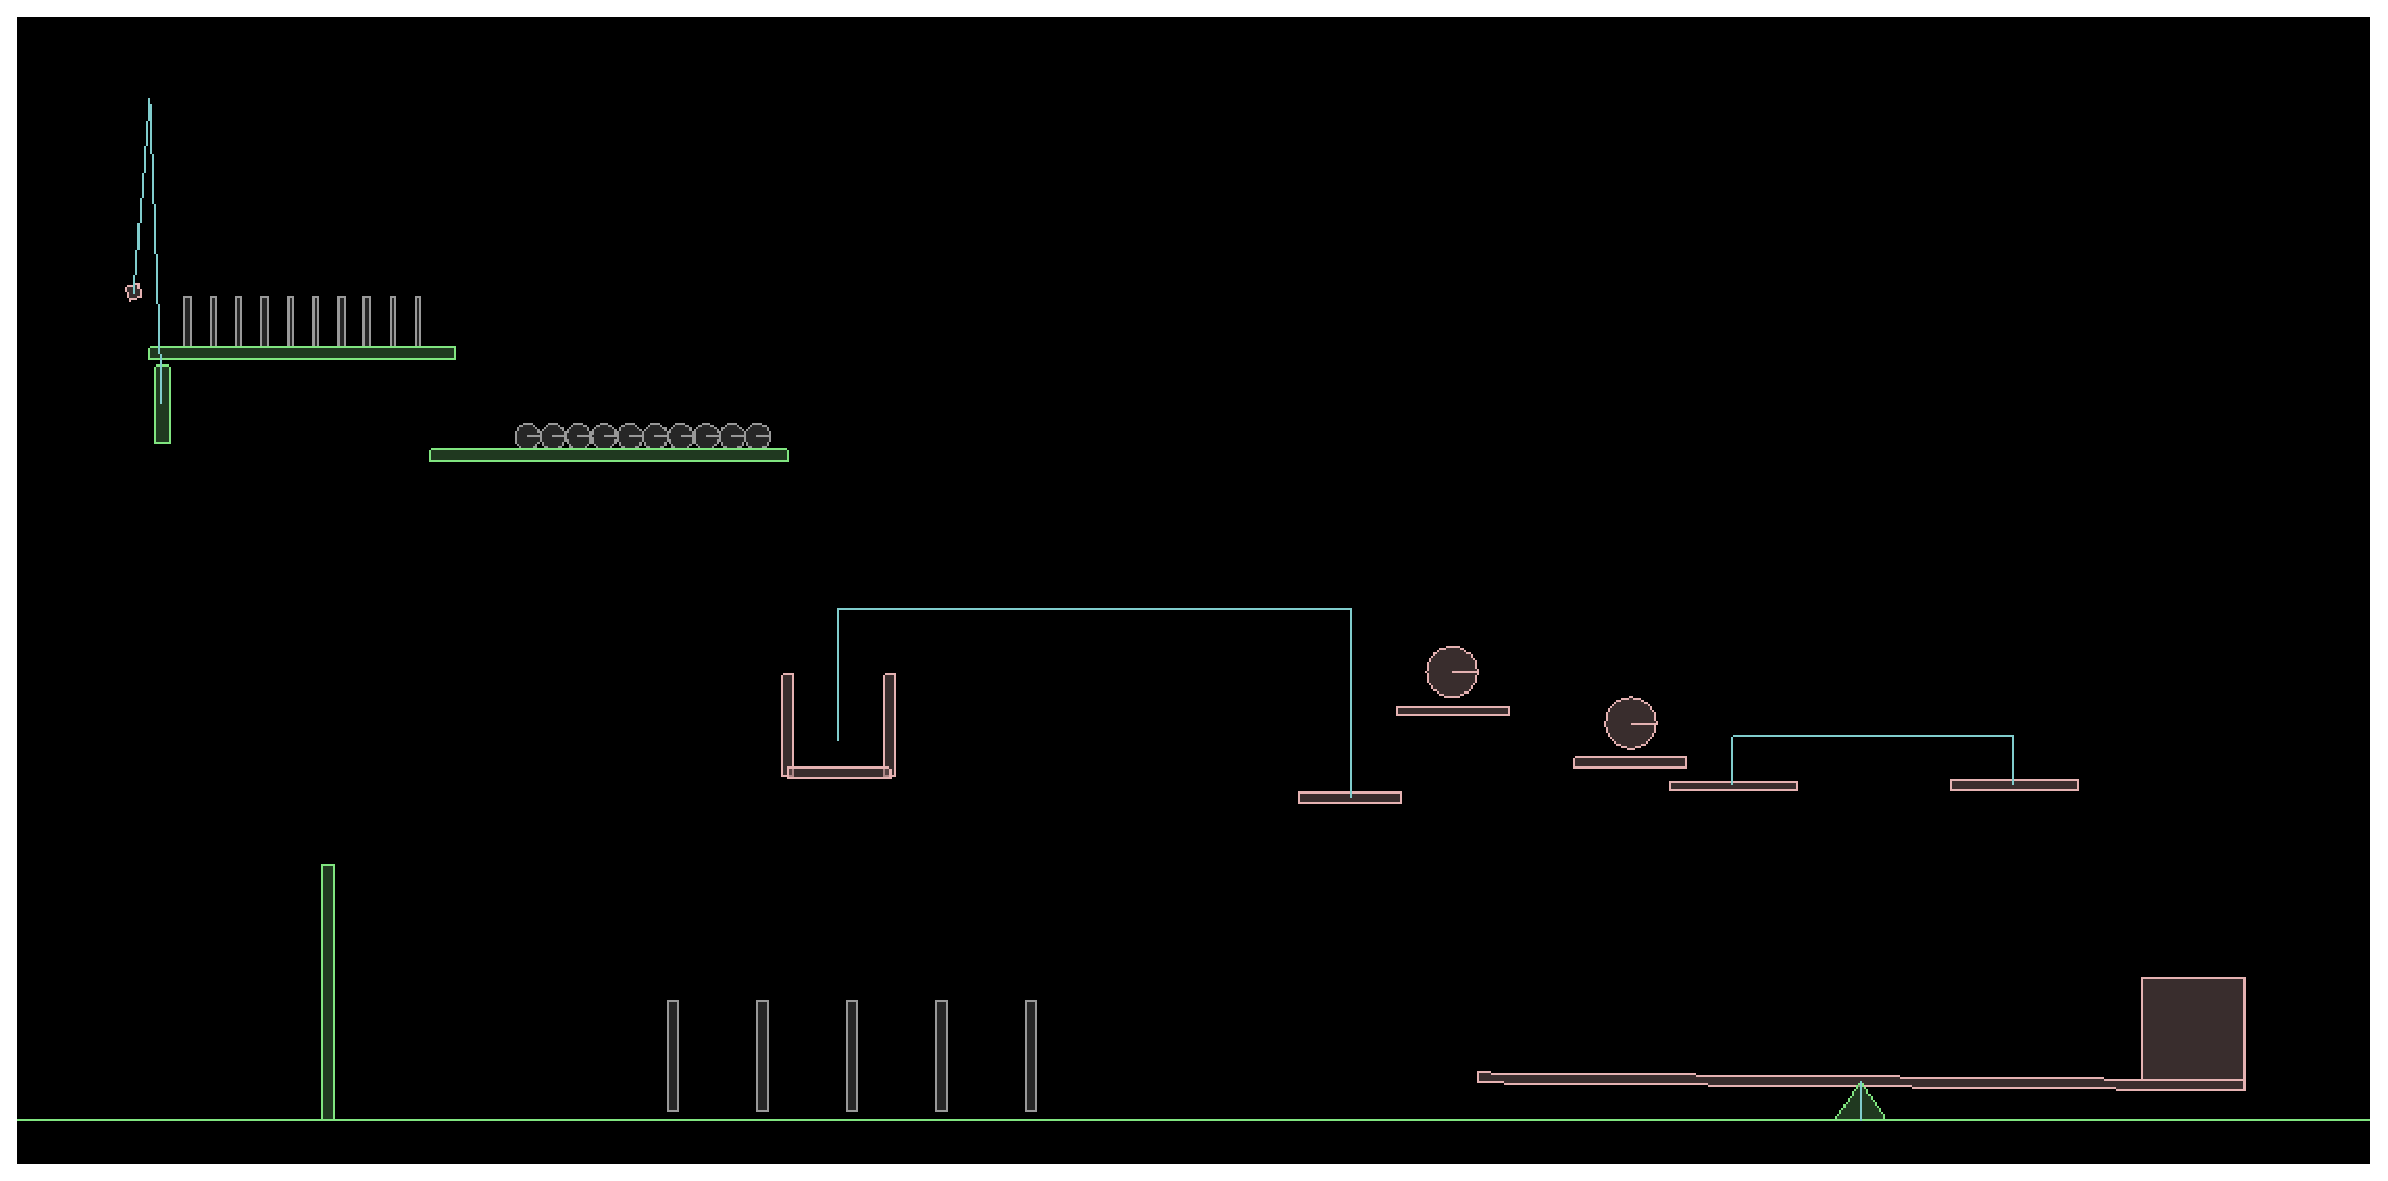
\includegraphics[scale=.33]{initial}
    \caption{Initial configuration of the system.}
\end{figure}
\subsection{Rotating horizontal platform with heavy sphere on it and the pulley system}
\begin{figure}[h!]
\centering
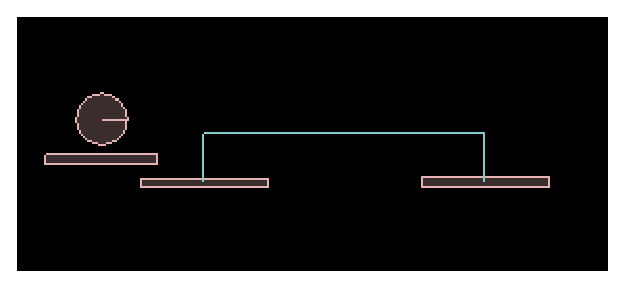
\includegraphics[scale=1]{rotatingplatform}
\caption{The heavy sphere rests on a free-to-rotate platform next to the pulley system}
\end{figure}
\indent \par{Initially the system is at rest and net force(F) is zero\cite{wikilaw2}. When the light box on the see-saw lands on the right platform of the pulley, the pulley system is imbalanced. As now the right side is heavier, the left platform moves up and disturbs the rotating platform, which in turn disturbs the heavy sphere.}
\\
\indent Initially, for all bodies, $\vec{F}$ denote the net force (in Newtons),
\begin{equation}
\vec{F}= 0
\end{equation}
\indent Let $m_{left}, m_{right}, m_{box}$ denote the masses(in kg) of the left platform, right platform and the light box, and let $\vec{g}$ denote the acceleration(in $m/s^2$) due to gravity. Then assuming frictionless pulley joints, the acceleration(in $m/s^2$) $\vec{a_1}$ of the system is given by Newton's second law of motion\cite{wikilaw2}
\begin{equation}
m_{right}\vec{g} + m_{box} \vec{g}- m_{left} \vec{g} = (m_{left}+m{right}+m_{box})\vec{a}
\end{equation}
\indent The value of acceleration $\vec{a}$ is not needed. We just need to understand that the left side of the pulley will rise and will disturb the heavy sphere.

\subsection{Rotating bars at the bottom}
\indent \par{There are 5 bars at the bottom which are free to rotate about their pivoted center.}
\begin{figure}[h!]
\centering
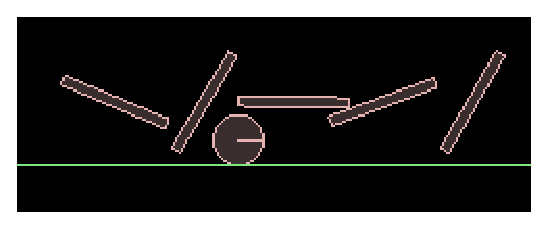
\includegraphics[scale=1.3]{bottombars}
\caption{Bars (initially vertical) being disturbed by the heavy sphere.}
\end{figure}
\\
\indent Let $m_{bar}, l_{bar}$ denote the mass(in kg) and length(in m) of each bar. If a bar is rotating with angular velocity $\vec{\omega_{i}}$ (in rad/s) and a sphere of mass $m_{sphere}$(in kg) travelling with velocity $\vec{v_{i}}$ (in m/s) hits it, then by conservation of angular momentum\cite{wikicoam} about the pivot point: 
\begin{equation}
m_{bar} \frac{l^2}{12} \vec{\omega_{i}} + m_{sphere} \vec{v_{i}} \frac{l}{2} = m_{bar}\frac{l^2}{12}\vec{\omega_{f}} + m_{sphere}\vec{v_{f}}\frac{l}{2}
\end{equation}
\\ \indent Here the $\vec{v_{f}} and \vec{\omega_{f}}$ denote the final velocity(in m/s) of sphere and angular velocity(in rad/s) of bar.
\\ If the coefficient of restitution\cite{wikirest} is $e$ (dimensionless) then we have, 
\begin{equation}
e(\vec{v_{i}}-\frac{l}{2}\vec{\omega_{i}}) =  \vec{v_{f}} - \frac{l}{2} \vec{\omega_{f}}
\end{equation}

\subsection{Vertical wall on bottom left}

\indent The coefficient of restitution of this wall is set to 5 (which is a bit unrealistic, but leads to interesting physics). 
\\ \indent If the coefficient of restitution\cite{hcv} is $e$ (dimensionless), and a sphere of mass $m_{sphere}$(in kg) hits this wall with velocity $\vec{v_{i}}$(in m/s) then the final velocity of sphere is given by\cite{rh} $\vec{v_{f}}$(in m/s) 
\begin{equation}
e\vec{v_{i}} = \vec{v_{f}}
\end{equation}
\begin{figure}[h!]
\centering
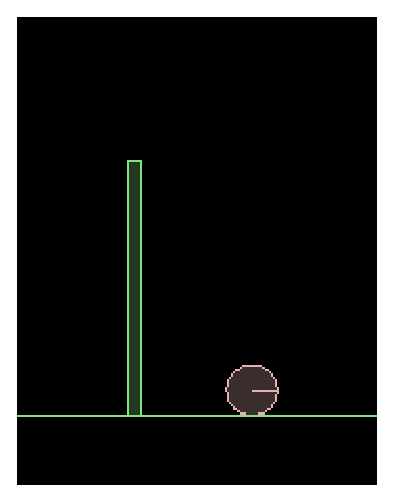
\includegraphics[scale=1.1]{verticalwall}
\caption{Fixed vertical wall.} 
\end{figure}

\section{Conclusion}
\indent The purpose of this assignment was to get familiar with Doxygen documentation and Latex. It also familiarized us with basics of Box2D. Simple physics concepts were applied on various components of the simulation. If you encounter any mistakes, please notify the authors.
\bibliographystyle{plain}
\bibliography{cs296_report_09}
\end{document}
